\chapter{Introduction}

\section{Introduction}
\subsection{Introduction to Invoice}
An invoice is a document that lists the products and 
services a business provides to a client and establishes 
an obligation on the part of the client to pay the 
business for those products and services.

Invoices are the backbone of the accounting system for 
small businesses.
\begin{figure}[h]\centering
	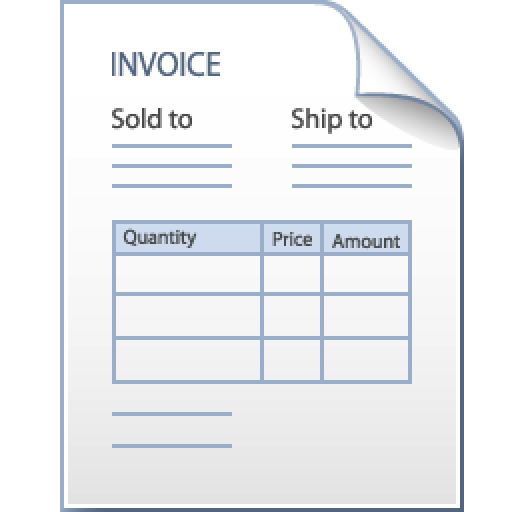
\includegraphics[width=2in]{invoice-template.png}
	\caption{A sample Invoice}\label{invoice-template}
\end{figure}

Invoices constitute some of the most valuable documents exchanged between business
partners, including government institutions. Companies exchange enormous number of
invoices daily, both in electronic and paper formats. The real obstacle lies on how efficiently and quickly the invoicing process is handled from order initiation to delivery and payment for goods or services. An invoice management system helps to simplify and
organise this process and thereby enhance process transparency.

The invoice management system generates, sorts and classifies invoices automatically.
It also monitors invoice status and sends notifications where necessary. Invoices are
automatically archived for the long term. With invoice management structures in place,
the quality of invoice data is improved.

Although invoices can be issued in a traditional printed format, e-invoicing provides methods of invoice transmission and processing via electronic means. The major difference
between e-invoices and traditional paper invoices is the automated process involved in
e-invoices.

\subsection{Problem Statement}
Invoice application being the basic need for all business, yet the software required for this purpose needs to be purchased from some software company. This creates the problem if any modifications are need to be brought to taxation methods or if any features needs to be added to meet some requirement.

Generally the invoice applications available today are just offline applications simply storing the billing info in local database. This is a drawback in the era of internet world, where people expect to get all information online regarding their purchasing details, due payments.


\section{About Project}
In this project, we have implemented a general purpose invoice web application where any user can create a profile and use it create invoices for their requirement

Since, its a web application all data and information are stored in online database server . It also has the advantage of easy updates if needed.

In this Invoice Web Application users first need to create their profile and then can add the items involved in their business along with the details of stocks and prices. 

It has features such as:
\begin{itemize}
\item Get the invoice in pdf format, which can be printed if needed.
\item Invoice history is maintained for each customer.
\item Customer details about due in their payments are maintained.
\item A copy of invoice in pdf format is sent to the customer email.\\[0.5cm]
\end{itemize}

\section{Aim and Scope}
\subsection{Aim}
To create a general purpose invoice web application where any user can conveniently utilize it to create invoices and can store all the details online and to provide modern web app features.
\subsection{Scope}
All the businesses irrespective of the levels of business either it may be distributors or retailers who have wide range of customers necessarily require an elegant and user-friendly invoice application in order for the smooth conduction of their business. Thereby it becomes a need and demand for an Invoice Application.\\[0.5cm]


\section{Objectives}
The main objective of this project is to overcome the drawback of traditional invoice application and to provide a modern general purpose invoice web application available for any user to conveniently create invoices. Also, maintain customer details to provide features regarding their due payments and invoice history.